\documentclass{article}

\usepackage{caption}
\usepackage{color}
\usepackage{fancyvrb}
\usepackage{geometry}
\usepackage{graphicx}
\usepackage{verbatim}
\usepackage{url}

\newcommand\ch[1]{\textcolor[rgb]{0,0,1}{\textbf{#1}}}

\newcommand{\timetbl}[4]{\par\vspace{5mm}\begin{tabular}{ l l l l }
Estimated Completion Date: & #1 & Estimated Completion Time: & #2 \\
Actual Completion Date: & #3 & Actual Completion Time: & #4 \\
\end{tabular}}

\title{Celeriac: A Daikon .NET Front-End}
\author{Developer Manual}

\begin{document}
\maketitle

\section{Introduction}
Daikon is a tool that infers likely program invariants from program traces \cite{DaikonUserManual:Online}. The Daikon tool relies on front-ends, such as the Chicory front-end for Java, to generate program traces for input. Celeriac is the first Daikon front-end for the .NET languages --- C\#, VB.NET, and F\#. This document describes the architecture of Celeriac, a Daikon Front-End for .NET.
\subsection{Instrumented Program}
Celeriac creates a binary with instrumentation calls added, which will produce a Daikon trace file (described below) when executed. Celeriac can be configured to execute the instrumented program directly from memory (\emph{online-mode}), or to save the instrumented program to disk (\emph{offline-mode}).

\subsection{Daikon Declaration File}
The first part of a Daikon trace file is called the declaration component, which is metadata describing the schema of each program point (method entrance or exit). While Celeriac is inserting instrumentation calls the \texttt{ILRewriter} (described in section \ref{il-rewriter}) also makes calls to the \texttt{DeclarationPrinter} class which writes the declaration portion of the trace file, as described in Section \ref{decl-printer}.

\subsection{Daikon Trace File}
The second component, the trace component, is not output by Celeriac directly. Instead it will be written by the program as it executes. When the IL rewriter is finished, it returns a memory stream which the front-end loads and executes, or saves to disk if desired.

\section{Design Goals}
\label{design-goals}
This section describes the design goals guiding the development of the .NET Daikon front-end.

\subsection{Work with any .NET program.}
While Celeriac will likely be used mainly with C\# programs, we leverage the Common Language Runtime architecture to make the front-end work with many .NET languages. Celeriac has been successfully used on F\# and VB.NET  programs. This compatibility is achieved by targeting the tool at binary programs (which are in CIL), as opposed to targeting source code.
\\ \\
However, Celeriac must specially detect the presence of some language-specific constructs, to enable detection of meaningful properties. For example, F\# uses its own list type instead of the .NET \texttt{System.Collections.List} type. To capture meaningful invariants over lists, such as the length of a list, or whether its elements are sorted, Celeriac treats a variable as a List if it has the \texttt{System.Collections.List} or the \texttt{FSharp.List} type.

\subsection{Don't require modification of the developer's build process.}
Commercial build processes can become very complex over time. As a result, it may be unwieldy or even impossible to integrate new tools into the build chain. An added benefit of meeting this design goal is that Celeriac can run on programs even when the source is not available, although the debugging symbols are necessary.

\subsection{Don't modify files on disk.}
Modifying the contents of the disk to instrument the program, e.g., creating a patched version of the executable, is similarly undesirable. The creation or replacement of binary files opens the door for versioning issues such as accidentally running an instrumented binary with incorrect options. Celeriac solves this problem by modifying the assembly, specifically adding the instrumentation calls, in memory and then executing the modified assembly directly from memory.
\\ \\
There are some situations where meeting this goal isn't possible. For example, when Celeriac creates an instrumented library that will be used by other programs, the instrumented library must be saved to disk. Also, when Celeriac is run on GUI programs using Windows Presentation Foundation (WPF), Celeriac must be run in off-line mode. This is because WPF programs resource loading process cannot complete when the program is in online mode, since the subject program is loaded into the Celeriac launcher's \texttt{AppDomain}. The program will then attempt to resolve resources from the Celeriac launcher's resources, but the resources exist only in the WPF application.

\section{Tool Architecture}
The front-end has two major components: an IL rewriter that inserts instrumentation calls into procedures and a run-time system that, when called from the subject program, outputs variable values to construct a Daikon trace file in the Daikon format.

\subsection{IL Rewriter}
\label{il-rewriter}
The IL rewriter is implemented in \texttt{ILRewriter.cs} and rewrites .NET binaries by inserting calls to the Celeriac runtime library. It utilizes the CCIMetadata IL Rewriting library\footnote{https://ccimetadata.codeplex.com/}. The CCIMetadata library provides an API for reading and writing CIL code using C\#. CCI also handles resolution of class and method references.
 %The IL rewriter component of the application, named \texttt{ILRewriter}, was adapted from a CCIMetadata example program that printed the name of local variables.
 The rewriter loads a .NET assembly in memory, walks over the IL and inserts instrumentation calls at the entrance and every exit of methods. The following figure illustrates the IL rewriter component.

\begin{center}
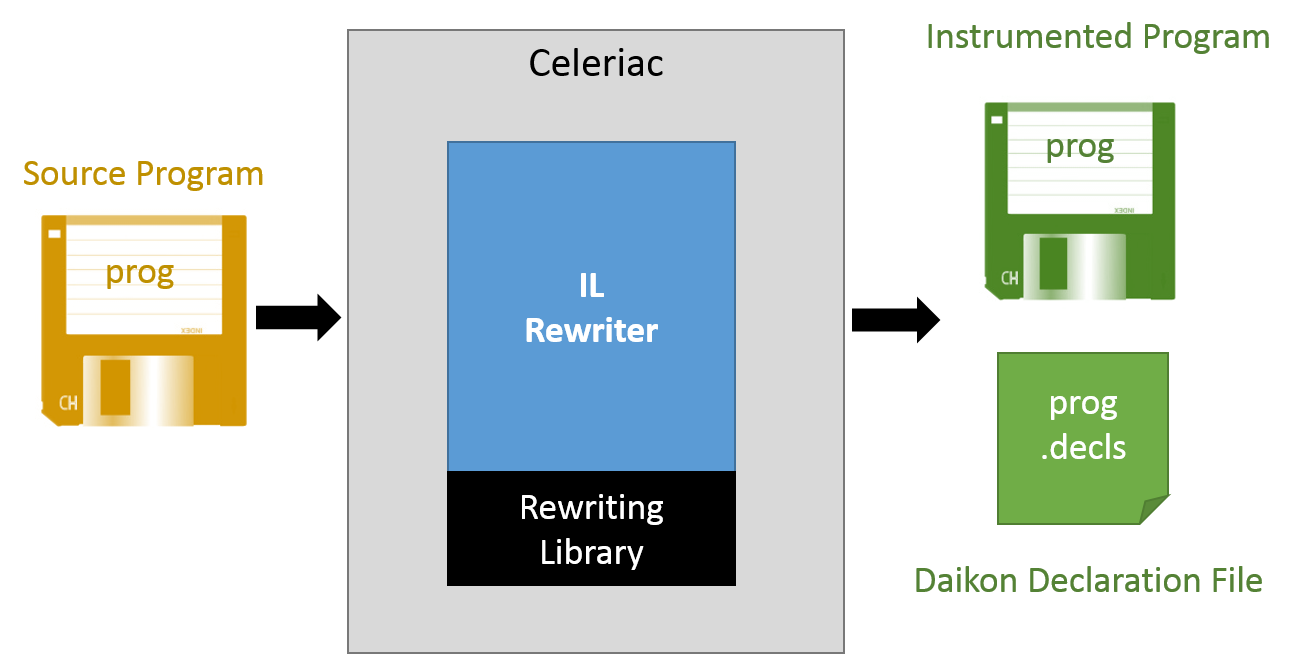
\includegraphics[scale=.7]{Arch1}
\end{center} \captionof{figure}{The IL Rewriter adds instrumentation calls to the source program and outputs expression metadata to be consumed by Daikon}

\subsection{Declaration Printer}
\label{decl-printer}
While performing IL rewriting to create an instrumented program Celeriac simultaneously builds the declaration component of the Daikon trace file. This is handled in the \texttt{DeclarationPrinter} class. Whenever Celeriac inserts an instrumentation call for a method, say \texttt{foo()}, it also writes to the declaration file a program point for the entry \texttt{foo()} and a listing of its parameters if any, and the receiver's fields and pure methods.

\subsection{Runtime Library}
The runtime library creates the actual trace file that will be input to Daikon. The main method exposed to source programs prints the name of a variable, and its value, then prints the name and value of each of that variables fields, pure methods, and elements if any. The following figure illustrates the functionality of the runtime library component.

\begin{center}
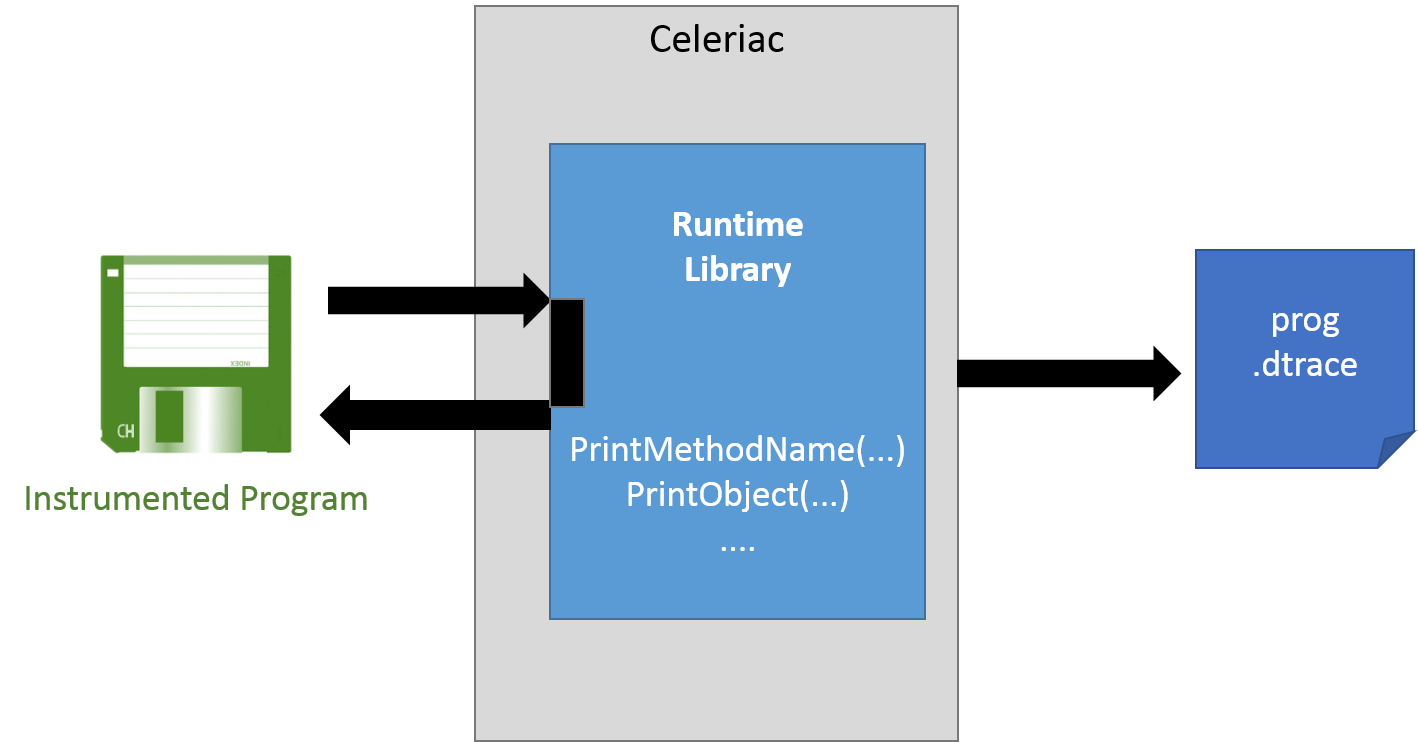
\includegraphics[scale=.7]{Arch2}
\end{center} \captionof{figure}{The runtime library contains instrumentation methods that are called by the modified source program. When called the methods write entries to a trace file, to be consumed by Daikon.}
\~ \\

The runtime library is implemented in the \texttt{VariableVisitor} class. When the \texttt{VisitVariable()} method is called from the instrumented program the value of the variable itself is printed. Then any static or instance fields of that variable, which are visited reflectively based on the declared type of the variable, are also printed. The instrumentation code traverses data structures and enumerates variables that implement the IList, ISet, or Dictionary interfaces, or their F\# equivalents.

%\section{Risks}
%This section describes the aspects of the project that are the riskiest, that is parts of the project may be difficult to complete during the fall (or at all).

%\paragraph{Instrumenting Exception Return Points}
%The instrumentation calls that the unmanaged profiler adds must maintain the validity of the MSIL code. For function prologues, this maintaining validity is apparently easy. For intermediary return points and exceptional return points, this is not trivial \cite{Mikunov:2003:Online}.

%\paragraph{Detecting / Instrumenting Complex Language Features}
%Certain language features, such a closures, may be compiled into weird
%constructs in the MSIL. It may be hard or impossible to detect all of
%these features in the MSIL code an instrument them accordingly.

\section{Design Decisions}
This section describes important design decisions, the alternatives, and the justification for the implemented choice.

\subsection{Type Resolution}
A Daikon front-end needs to print out each the same list of fields and pure methods for a variable fields at every instance of a program point. This is a requirement of Daikon, and exists because Daikon outputs invariants that are always true. If a variable were present at some instances of a program points but not others then Daikon would not be able to reason about that variable.
\\ \\
This means a front-end needs to know the declared type of each variable, rather than the run-time type, which may be different each time a method is called, and not available at instrumentation time, when the declaration file is printed.
\\ \\
There are several possible approaches for identifying the declared type of each variable:

\begin{itemize}
  \item Inspect the source code as text, and manually parse the program to learn each expression's type.
  \item Mimic or operate with the code compiler, since it must already determine each expression's type, and to use this result.
  \item Extract declared types from a binary program using a bytecode or metadata library.
  \item Perform reflection on the binary program, in a structured search to match field names to a list of fields extracted via reflection, which would contain their declared types.
\end{itemize}

Celeriac uses the metadata library approach. Celeriac uses the CCIMetadata library \cite{cci} to determine the types of each variable, albeit in a type system constructed by CCI, that does not have information, such as the fields of the type. The fields of the type are available in the .NET Type, so a bridge between these two type systems must be created. This is accomplished through the use of assembly-qualified name \cite{aqn}. An assembly-qualified name uniquely identifies a type, and allows the Type to be retrieved at run-time.
\\ \\
The complication with this approach is to build the appropriate assembly-qualified name given a CCIType. This especially problematic for generic types that may have multiple bounds, e.g. \texttt{public addEdge<TEdge>(TEdge edge) where TEdge : IEdge<TVertex>, IComparable<TEdge>, IPrettyPrintable}. Generics are reified at runtime in .NET, so at runtime a type \texttt{TEdge} that implements all necessary interfaces would be created, but this type isn't available at instrumentation time, when it is needed by Celeriac. The class \texttt{CeleriacTypeDeclaration} compensates for this, and can be constructed so that a declared type is actually of a list of types, which are a list of constraints on a generic expression. In the code presented above the declared type of the parameter \texttt{edge} would be a list of its generic constraints: \texttt{IEdge<TVertex>, IComparable<TEdge>, IPrettyPrintable}.  
\\
The implementation of the type resolution, which is in \texttt{TypeManager.cs}, was difficult to complete, with bugs appearing over many months of the development. The difficulty resulted from the complex structure of CCI's representation of the .NET type system. The CCI type system does not correspond closely to the .NET one for the purposes of creating assembly qualified names. For example, types of class generics and method generics appear the same in assembly qualified names, but are very different C\# types. Running Celeriac on the test suite for the Mono C\# compiler\footnote{\url{http://www.mono-project.com/CSharp_Compiler}} provided high confidence that the resulting type resolution system is correct.
\\ \\
We chose the metadata approach over alternatives because it fit best with the design goals (discussed earlier in Section \ref{design-goals}. Source code parsing alternatives would not be feasible because they fail the design goals of allowing Celeriac to run on multiple languages and being build processes independent (since they require source code). Compiler interop would also fail the build process independence goal, and would be infeasible as well because most .NET code uses Microsoft's proprietary compiler.

\subsection{Instrumentation Granularity}
Celeriac inserts instrumentation calls to print out all appropriate fields for a given object. This means Celeriac inspects each object's type twice, once at instrumentation time to print the declaration file, and again at runtime. This process involves examining an object's type, determining which fields to print, and then printing either a declaration (when the program is instrumented) or printing the value (when the program is run).
\\ \\
An alternative would insert calls to print the field values directly, and perform
no inspection at runtime. The two figures below illustrate the practical difference.
\begin{center}
\begin{Verbatim}[commandchars=\\\{\}]
public void compare(Point p1,
                    Point p2) \{
	\ch{PrintObject(this);}
	\ch{PrintObject(p1);}
	\ch{PrintObject(p2);}
	... Client Code ...
\}
\end{Verbatim}
\end{center} \captionof{figure}{Instrumentation pseudo-code: the variable visitor is called for each parameter, including the receiver, but not directly on a variables's fields.}
\begin{center}

\begin{Verbatim}[commandchars=\\\{\}]
public void compare(Point p1,
                    Point p2) \{
	\ch{PrintField(this, �foo�);}
	\ch{PrintField(this, �bar�);}
        ... More Visitor Code ...
	... Client Code ...
\}

\end{Verbatim}
\end{center} \captionof{figure}{Alternative Instrumentation pseudo-code: the variable visitor is called for each parameter and variable's fields directly.}
\  \\
However, this choice was not implemented for three reasons. First, it would lead to a much greater increase in code size. Whereas Celeriac inserts 1 new method for each relevant variable (parameter, field, etc.), the proposed alternative would insert 1 new method for each new variable's fields, resulting in much larger instrumented programs. It would require many more context-switches between the client's program and Celeriac's runtime library. Finally, much more work being would be done in IL rather than managed C\#, and C\# is much easier to develop in.
% \subsection{Exceptional Post-Conditions}

\newpage
\begin{comment}
\appendix

\section{Appendix: Project Schedule and Milestones}
This section describes the project milestones and history.

\subsection{10/2010 - 12/2010}
Work began on the instrumentor this quarter. A first attempt was to use the unmanaged Profiler API. First C\# reflection was used to analyze the program, and then the Profiler API's function enter/leave hooks were used to output the appropriate variable information. Manually editing the MSIL was extremely difficult and error-prone, especially for methods with multiple exit points and exception handling, so this approach was abandoned.

A pure IL rewriting approach using the CCIMetadata Library was attempted, where the output program was saved to disk as a new executable, however this violated the Disk Modifications Avoidance design goal. A hybrid of the previous two methods was considered where the CCIMetadata Library would create the new MSIL, and this would be handed to the unmanaged Profiler, to be substituted for the original method IL.

A presentation of the work to this point was presented to the UW CSE PL\&SE group on December 13th.
\subsection{1/2011 - 3/2011}
The previously described method was almost immediately shown to be infeasible. The CCIMetadata rewritten code produced different method tokens than were present in the original program, and thus could not be used. The main developer on the CCIMetadata project confirmed this issue could not be resolved in context. Analysis of alternate methods for IL rewriting was completed. It was determined that using the program with instrumentation inserted by CCIMetadata, but loaded into memory and ran instead of written to disk was the best approach.

The remainder of the quarter was spend implementing the profiler and visitor, and getting them to conform to Daikon specification. At the conclusion of the quarter an alpha version of the front-end was functional, and could generate simple datatrace files that Daikon could process.

\subsection{4/2011 - 6/2011}
During this quarter reflective visiting and array-style visiting of IEnumerable types were implemented. Most command-line arguments available to Chicory were documented. A test suite was added, modeled off the Kavasir (C++) front-end test suite. Chicory test sources were transliterated from Java to C\# and ran through the front-end. Output invariants were compared to the invariants produced by Chicory, and bugs in the front-end were fixed to rectify the differences. Exception handling was also added, a feature new to Daikon front-ends.

\subsection{9/2011 - 12/2011}
During this quarter the first code review of Celeriac was completed, resulting in many name improvements. Celeriac was extended to output multiple method exits points for methods that return more than once. A Google Code issue tracker was established. Celeriac was extended to work on programs with multiple threads.

\subsection{1/2012 - 3/2012}
During this quarter Celeriac was extended to run on pure methods and with the first additional language, F\#. This introduced the complication that F\# uses its own lists, and special handling was added for these.

\subsection{4/2012 - 6/2012}
During this quarter Celeriac's collection support was significantly expanded, specifically to include both F\# and C\# Sets and Maps. As well, support for generic types with multiple constraints was added as well. The documentation was significantly updated.

\subsection{9/2012 - 12/2012}
During this quarter the test suite was expanded and enhanced. WPF programs were tested for the first time, as were VB.NET programs. These each introduced bugs, which were fixed. Support was added for using Celeriac on programs exercised by external testing systems such as the Visual Studio testing system and NUnit.

\subsection{1/2013 - 3/2013}
During this quarter Celeriac was expanded to run on large sample .NET programs, for the research paper. This included running Celeriac on programs in a variety of languages and types, e.g. libraries, GUI applications, etc. A new command line option for WPF programs was added. Bugs were fixed with elimination of jagged and multi-dimensional arrays and type issues. The --std-visiblity flag was significantly broken before, and revamped. Pure method instrumentation was improved. Celeriac was run on the Mono test suite, giving higher confidence in its robustness.

\subsection{4/2013 - 6/2013}
In this quarter much of the work was focused on wrapping up Celeriac, rather than implementation of new features. The first full release of Celeriac was prepared, and made on June 14. Developer and user documentation were updated and expanded. Many old issues were fixed for the release. Remaining issues were examined and received detailed explanations for new developers. A presentation on Celeriac was given to the PLSE group on May 17th.
\end{comment}


\begin{comment}
\subsection{Introductory Milestones - From the 10/2010 - 12/2010 section}

\subsubsection{Read the First Three Sections of the Daikon User Manual}
Read the first three sections of the Daikon Developer Manual \cite{DaikonUserManual:Online}. Perform the Java \verb|StackAr| example to get an idea of what Daikon can do and what it is like to use Daikon.

\timetbl{10/4/2010}{2 hours}{10/5/2010}{2 hours}

\subsubsection{Read the ``New Front Ends'' Section of the Daikon Developer Manual}
Read the ``New Front Ends'' section of the Daikon Developer Manual \cite{DaikonDeveloperManual:Online}

\timetbl{10/6/2010}{1 hour}{10/6/2010}{1 hour}

\subsubsection{Read the File Formats Appendix}
Read the ``File Formats'' appendix of the Daikon Developer Manual to get a clearer idea of the information that the front-end will have to output.

\timetbl{}{}{}{}

\subsubsection{Install Visual Studio 2010 Ultimate Edition from MSDNAA}
Download and install a copy of Visual Studio 2010 Ultimate Edition form the MSDNAA website. It is available for free. We have to use Visual Studio 2010 Ultimate Edition in order to use Microsoft Research's tools (e.g., the code contract framework).

\timetbl{10/6/2010}{1.5 hours}{10/6/2010}{1.5 hours}

\subsection{Profiler Milestones}

\subsubsection{Hello World}
Build an unmanaged profiler that logs "Hello World" to a file specified by the user via the command line whenever a program is run using the profiler.

\timetbl{10/17/2010}{7 hours}{10/17/2010}{8 hours}

\subsubsection{Function Names}
Modify the profiler to log the name of each function that is compiled by the JIT right before they are compiled.

\timetbl{10/25/2010}{15 hours}{}{}

\subsubsection{Function Names 2.0}
Modify the profiler to insert a prologue in each function that outputs the name of the function to the log whenever it is called.
We decided we didn't need to do a prologue after all.
\timetbl{}{}{}{}

\subsubsection{Parameter Names}
Modify the profiler to insert a prologue in each function that outputs the names of the function parameters to the log whenever it is called.
Didn't end up using a prologue, instead use reflection to output function parameter names to a file, then parse those in the profiler.
\timetbl{}{}{11/11/2010}{22 hours}

\subsection{Instrumentation Milestones}

This section was left intentionally blank
\end{comment}
\newpage
\bibliographystyle{plain}
\bibliography{daikon-dotnet}

\end{document}


